\documentclass[12pt]{article}

\usepackage[utf8]{inputenc}
\usepackage{listings}
\usepackage{graphicx}
\usepackage{float}
\usepackage{geometry}
\usepackage{authblk}
\usepackage{setspace}

\newcommand*{\TitleFont}{
  \usefont{\encodingdefault}{\rmdefault}{b}{n}
  \fontsize{30}{40}
  \selectfont}

\usepackage{parskip}
\setlength{\parskip}{1.0\baselineskip plus2pt minus2pt}
%% \setlength{\baselineskip}{1cm}

\addtolength{\topmargin}{-50pt}
\addtolength{\textheight}{130pt}
\addtolength{\textwidth}{95pt}
\addtolength{\oddsidemargin}{-45pt}

\title{\TitleFont{Computação Gráfica}}
\author{David Gomes (2013136061) \and \vspace{-0.1cm} André Baptista (2013136742)}
\date{}

\begin{document}
\maketitle

\section*{Introdução}
O nosso projeto de Computação Gráfica consiste num ambiente 3D com várias bolas a movimentar-se
dentro de um cubo coberto, na sua base, por água.

\begin{figure}[H]
  \centering
  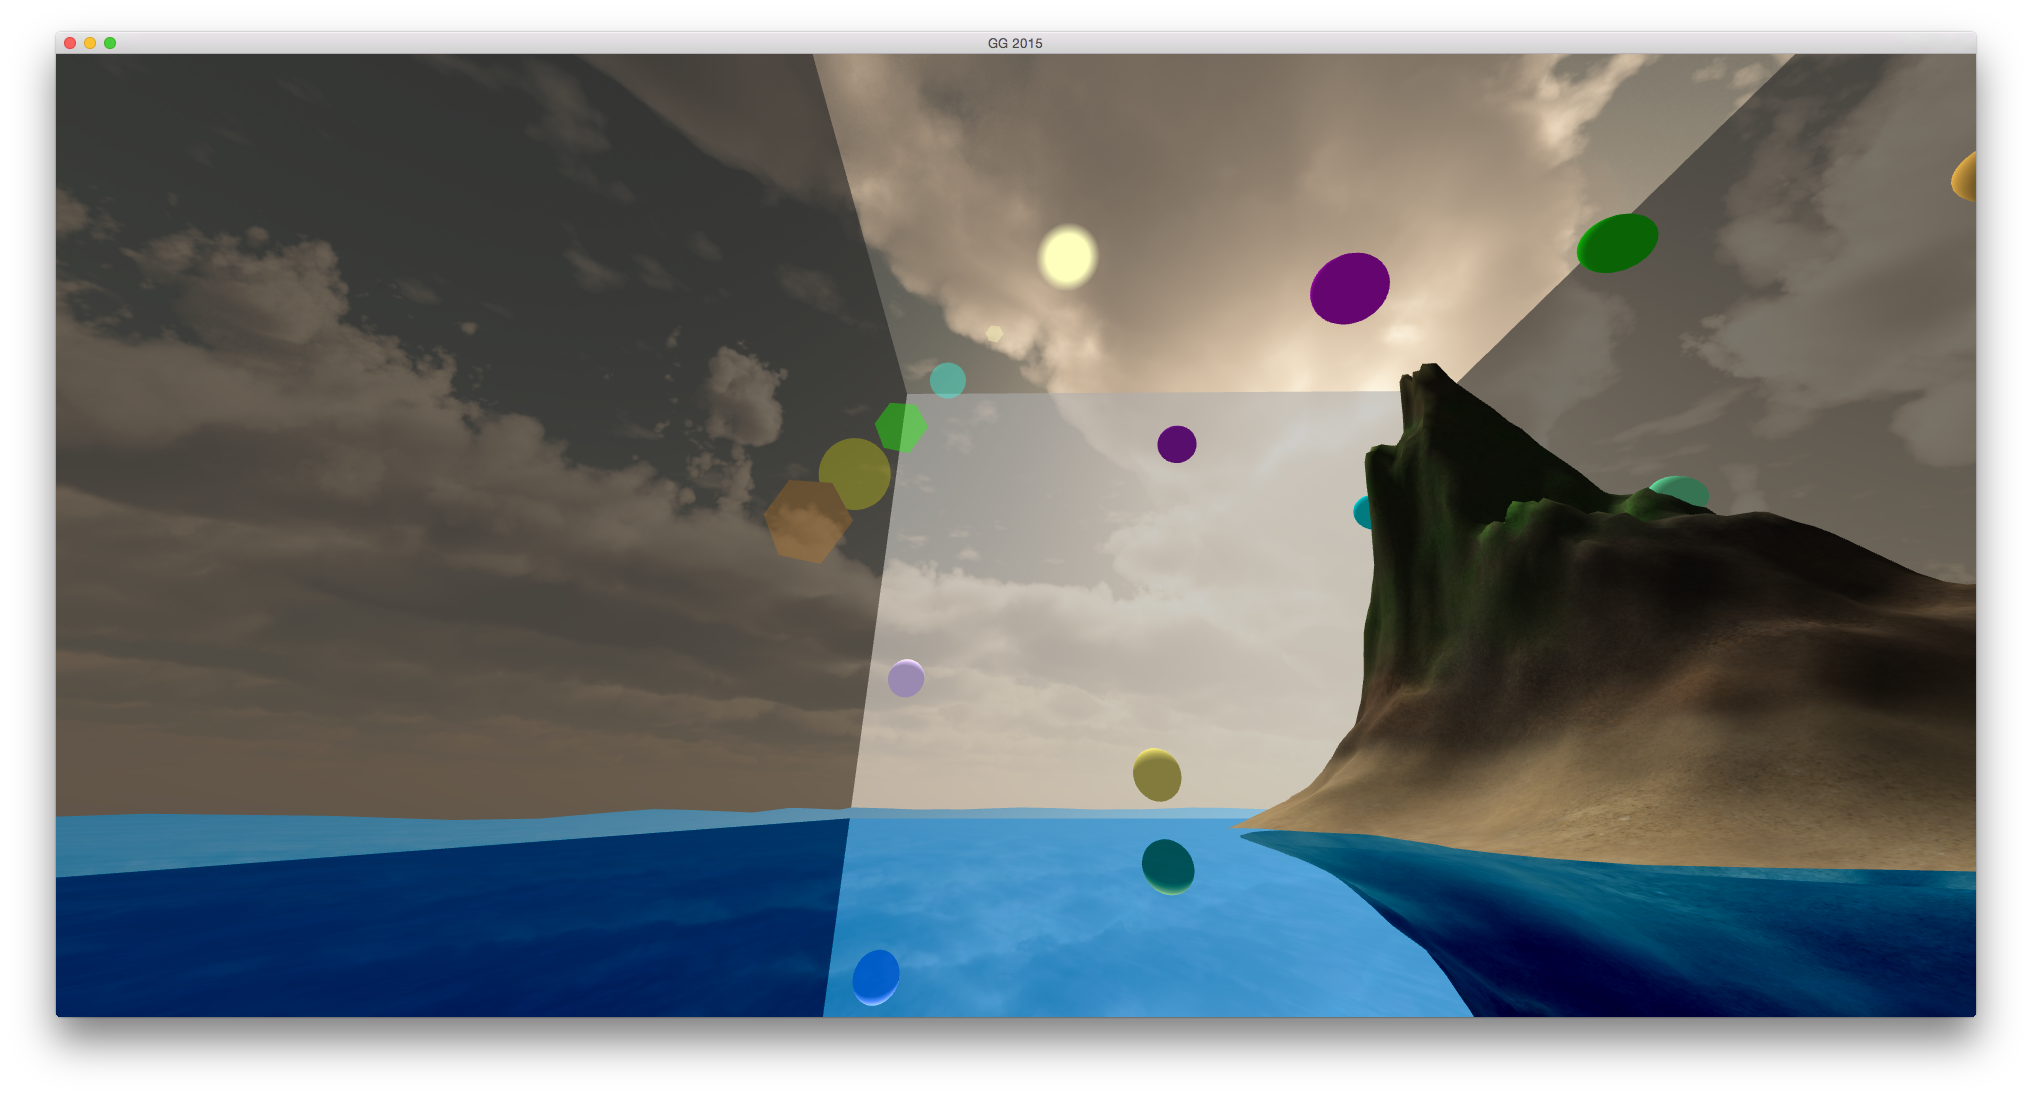
\includegraphics[width=0.75\textwidth]{screenshot}
\end{figure}

\section*{Features}
\subsection*{Object Loader}
Para facilitar o desenvolvimento do projeto criamos um \textit{loader} de objetos que desenha modelos
a partir de ficheiros \texttt{.obj}. Com este mecanismo associado à classe \texttt{Object}, carregamos o modelo da ilha assim como o do cubo.
\subsection*{Sol}
\subsection*{Reflexão}
\subsection*{Água}
\subsection*{Lens Flare}
\subsection*{Colisões}
\subsection*{Explosões (partículas)}
\subsection*{Lançamento de Bolas}

\end{document}